\documentclass[letterpaper,11pt]{article}
\usepackage{graphicx}
\usepackage{listings}
\usepackage[super]{nth}
\usepackage[hyphens]{url}
\usepackage{hyperref}
\usepackage{amsmath}
\usepackage[makeroom]{cancel}
\usepackage[table]{xcolor}
\usepackage{comment}
\usepackage[space]{grffile}
\usepackage{csvsimple}
\usepackage{longtable}


\newcommand*{\srcPath}{../src}%

\lstset{
	basicstyle=\footnotesize,
	breaklines=true,
}

\begin{document}

\begin{titlepage}

\begin{center}

\Huge{Assignment 6}

\Large{CS 532:  Introduction to Web Science}

\Large{Spring 2017}

\Large{Grant Atkins}

\Large Finished on \today

\end{center}

\end{titlepage}

\newpage


% =================================
% First question
% =================================
\section*{1}

\subsection*{Question}

\begin{verbatim}
1.  D3 graphing (10 points)

Use D3 to visualize your Twitter followers.  Use my twitter account
("@phonedude_mln") if you do not have >= 50 followers.  For example,
@hvdsomp follows me, as does @mart1nkle1n.  They also follow each
other, so they would both have links to me and links to each other.

To see if two users follow each other, see:
https://dev.twitter.com/rest/reference/get/friendships/show

Attractiveness of the graph counts!  Nodes should be labeled (avatar
images are even better), and edge types (follows, following) should
be marked.

Note: for getting GitHub to serve HTML (and other media types), see:
http://stackoverflow.com/questions/6551446/
can-i-run-html-files-directly-from-github-instead-of-just-viewing-their-source

Be sure to include the URI(s) for your D3 graph in your report. 
\end{verbatim}

\clearpage
\subsection*{Answer}

First approaching this problem I decided to use the tweepy library for python 3.6 to retrieve a json formatted list of Dr. Nelson's followers, which for me at the time was 634 followers, which was then saved to a file named \textbf{phonedudeFollowers.json} using the python script \textbf{getFollowers.py} shown in Listing \ref{lst:getFollowers.py}. Then I decided to reduce the number of friendships to check since checking friendships between all 634 followers would have been fairly time consuming. Therefore I created another script called \textbf{chooseUsers.py} which would pick 100 random integers for numbers between 1 and 634, which would act as which line numbers I would choose to sample from the json followers I retrieved earlier. This method actually worked out very well because I ended up getting quite a few members that were actually at Old Dominion University, as shown in Table \ref{table:q1userschosen}, without me tampering with it at all - however I may have run it a few times to test it.

I then took the 100 followers I had just chosen, added Dr. Nelson's user name $phonedude\_mln$, and continued to use tweepy again to check friendships between this list of users using the python script \textbf{findFriendships.py} shown in Listing \ref{lst:friendships.py}. It should be noted that I first decided to minimize the number of api calls by reducing the pairs I had to check. This was done by the \textit{minimizeConnections} function, which mapped all users as keys with values of every other user that was not already a key. This reduced the number of api calls from 10100 to 5150, with more logic explained in that function starting on line 14. This script took a several hours due to Twitter's rate limits. When it was completed all the friendships to each other user was saved to \textbf{friendships.csv} in the format of:

\begin{table}[htb]
\centering
\begin{tabular}{ | l | l | l | l |}
\hline
\textbf{Source User} & \textbf{Target User} & \textbf{Following Target} & \textbf{Followed By Target} \\
\hline
\end{tabular}
\caption{Format of friendships.csv, where Following fields are booleans}
\label{table:q1csvtable}
\end{table}

Finally to utilize D3.js to its utmost, I decided to convert the csv data and json data saved earlier, to create a new formatted json data with two main keys: nodes and links. To accomplish this I created a script named \textbf{createGraphJson.py}, so the data could properly represent a force directed graph. The all followers graph shown in Figure \ref{fig:q1allfollwersgraph} and the friendship graph of the 100 users generated shown in Figure \ref{fig:q1friendshipgraph} were generated using D3 using the \textit{drawGraph} function defined in \textbf{twitterFriendship.js} shown in Listing \ref{lst:q1javascript}. On hover a side bar should appear showing the user's name, user id, and profile image which links to the associated account. It should be noted that 1 user on the friendship graph is disconnected because when tweepy checked the account it was actually suspended by the time it got to it, making friendships impossible to establish. These two visualizations can be found here:

\url{https://cdn.rawgit.com/grantat/cs532-s17/b410d0d7/assignments/A6/src/index.html}

%\begin{table}[htb]
%\centering
\begin{longtable}{ | l |}
\textbf{Chosen Followers} \\
\hline
Daniel \\
\hline
Ren� Voorburg \\
\hline
Brenda Berkelaar \\
\hline
Cassie Findlay \\
\hline
Hussam Hallak \\
\hline
British Library Labs \\
\hline
Space 3D 360� VR \\
\hline
Kh Talha \\
\hline
Angela Woodall \\
\hline
Fredericik Begbeder \\
\hline
Kevin Levrone \\
\hline
Christopher Chyr \\
\hline
Jessica Smith \\
\hline
Zhaohuan Wang \\
\hline
Michael Stevenson \\
\hline
Stephanie A Kingsley \\
\hline
Andrea Goethals \\
\hline
TEI Landmark \\
\hline
DBpedia \\
\hline
Hung V. Do \\
\hline
Gardner Campbell \\
\hline
Jacquelyn Clements \\
\hline
dinesh kumar paladhi \\
\hline
Alex Dolan-Mescal \\
\hline
psleeman \\
\hline
lyn maccorkle \\
\hline
Larry Wayne Wilson \\
\hline
WOSP Workshop \\
\hline
NetLab \\
\hline
Huan Huang \\
\hline
Karl Blumenthal \\
\hline
Archivportal-D \\
\hline
Kees Teszelszky \\
\hline
Mike Amundsen \\
\hline
OTL National Event \\
\hline
Shira Peltzman \\
\hline
Daniel Rehn \\
\hline
Matthew Weber \\
\hline
Kayla Fox \\
\hline
Alex Wade \\
\hline
IJDL \\
\hline
JCDL 2016 \\
\hline
Edward McCain \\
\hline
Naima \\
\hline
Kenneth E. Chapman \\
\hline
rudolf \\
\hline
Lam Mai ? \\
\hline
Lana Kinnie \\
\hline
Shamim \\
\hline
Bertram Lyons \\
\hline
J. Stoddert \\
\hline
Peter Murray \\
\hline
Jennifer Serventi \\
\hline
MD SHAJID \\
\hline
Paul Wheatley \\
\hline
?????? ????? \\
\hline
Jessica Ogden \\
\hline
gaurav \\
\hline
Stanford Libraries \\
\hline
Karen Hanson \\
\hline
DOWN at ODU \\
\hline
Jonathan Greenberg \\
\hline
Melissa Durham \\
\hline
Benn Joseph \\
\hline
Boaty McBoatface \\
\hline
Bergis Jules \\
\hline
CRISTIANO PLAMEN \\
\hline
B. Danette Allen \\
\hline
Ray Matthews \\
\hline
Peter Burnhill \\
\hline
Klaus Berberich \\
\hline
Nancy Alajarmeh \\
\hline
anaas \\
\hline
Mohamed Aturban \\
\hline
WS-DL Group, ODU CS \\
\hline
Gerhard Gossen \\
\hline
Robin C. Pike \\
\hline
ISRJ \\
\hline
Peter Webster \\
\hline
Yasmina Anwar \\
\hline
Robert H. McDonald \\
\hline
tpdl2017 \\
\hline
Juliane Stiller \\
\hline
Konrad Lischka \\
\hline
Baptiste Fluzin \\
\hline
Jak Akdemir \\
\hline
Aleph Archives \\
\hline
Mike Zarro \\
\hline
Ben LeBrun \\
\hline
Gina Jones \\
\hline
Mat Kelly \\
\hline
Frank McCown \\
\hline
Andy Jackson \\
\hline
Joan Smith \\
\hline
Scott Ainsworth \\
\hline
Moustafa Emara \\
\hline
Kaitlin L. Costello \\
\hline
Hany SalahEldeen \\
\hline
William J Nixon \\
\hline
Michele Weigle \\
\hline
\caption{Users generated from \textbf{chooseUsers.py}}
\label{table:q1userschosen}
\end{longtable}
%\end{table}

\clearpage
 \begin{figure}[h]
 \centering
 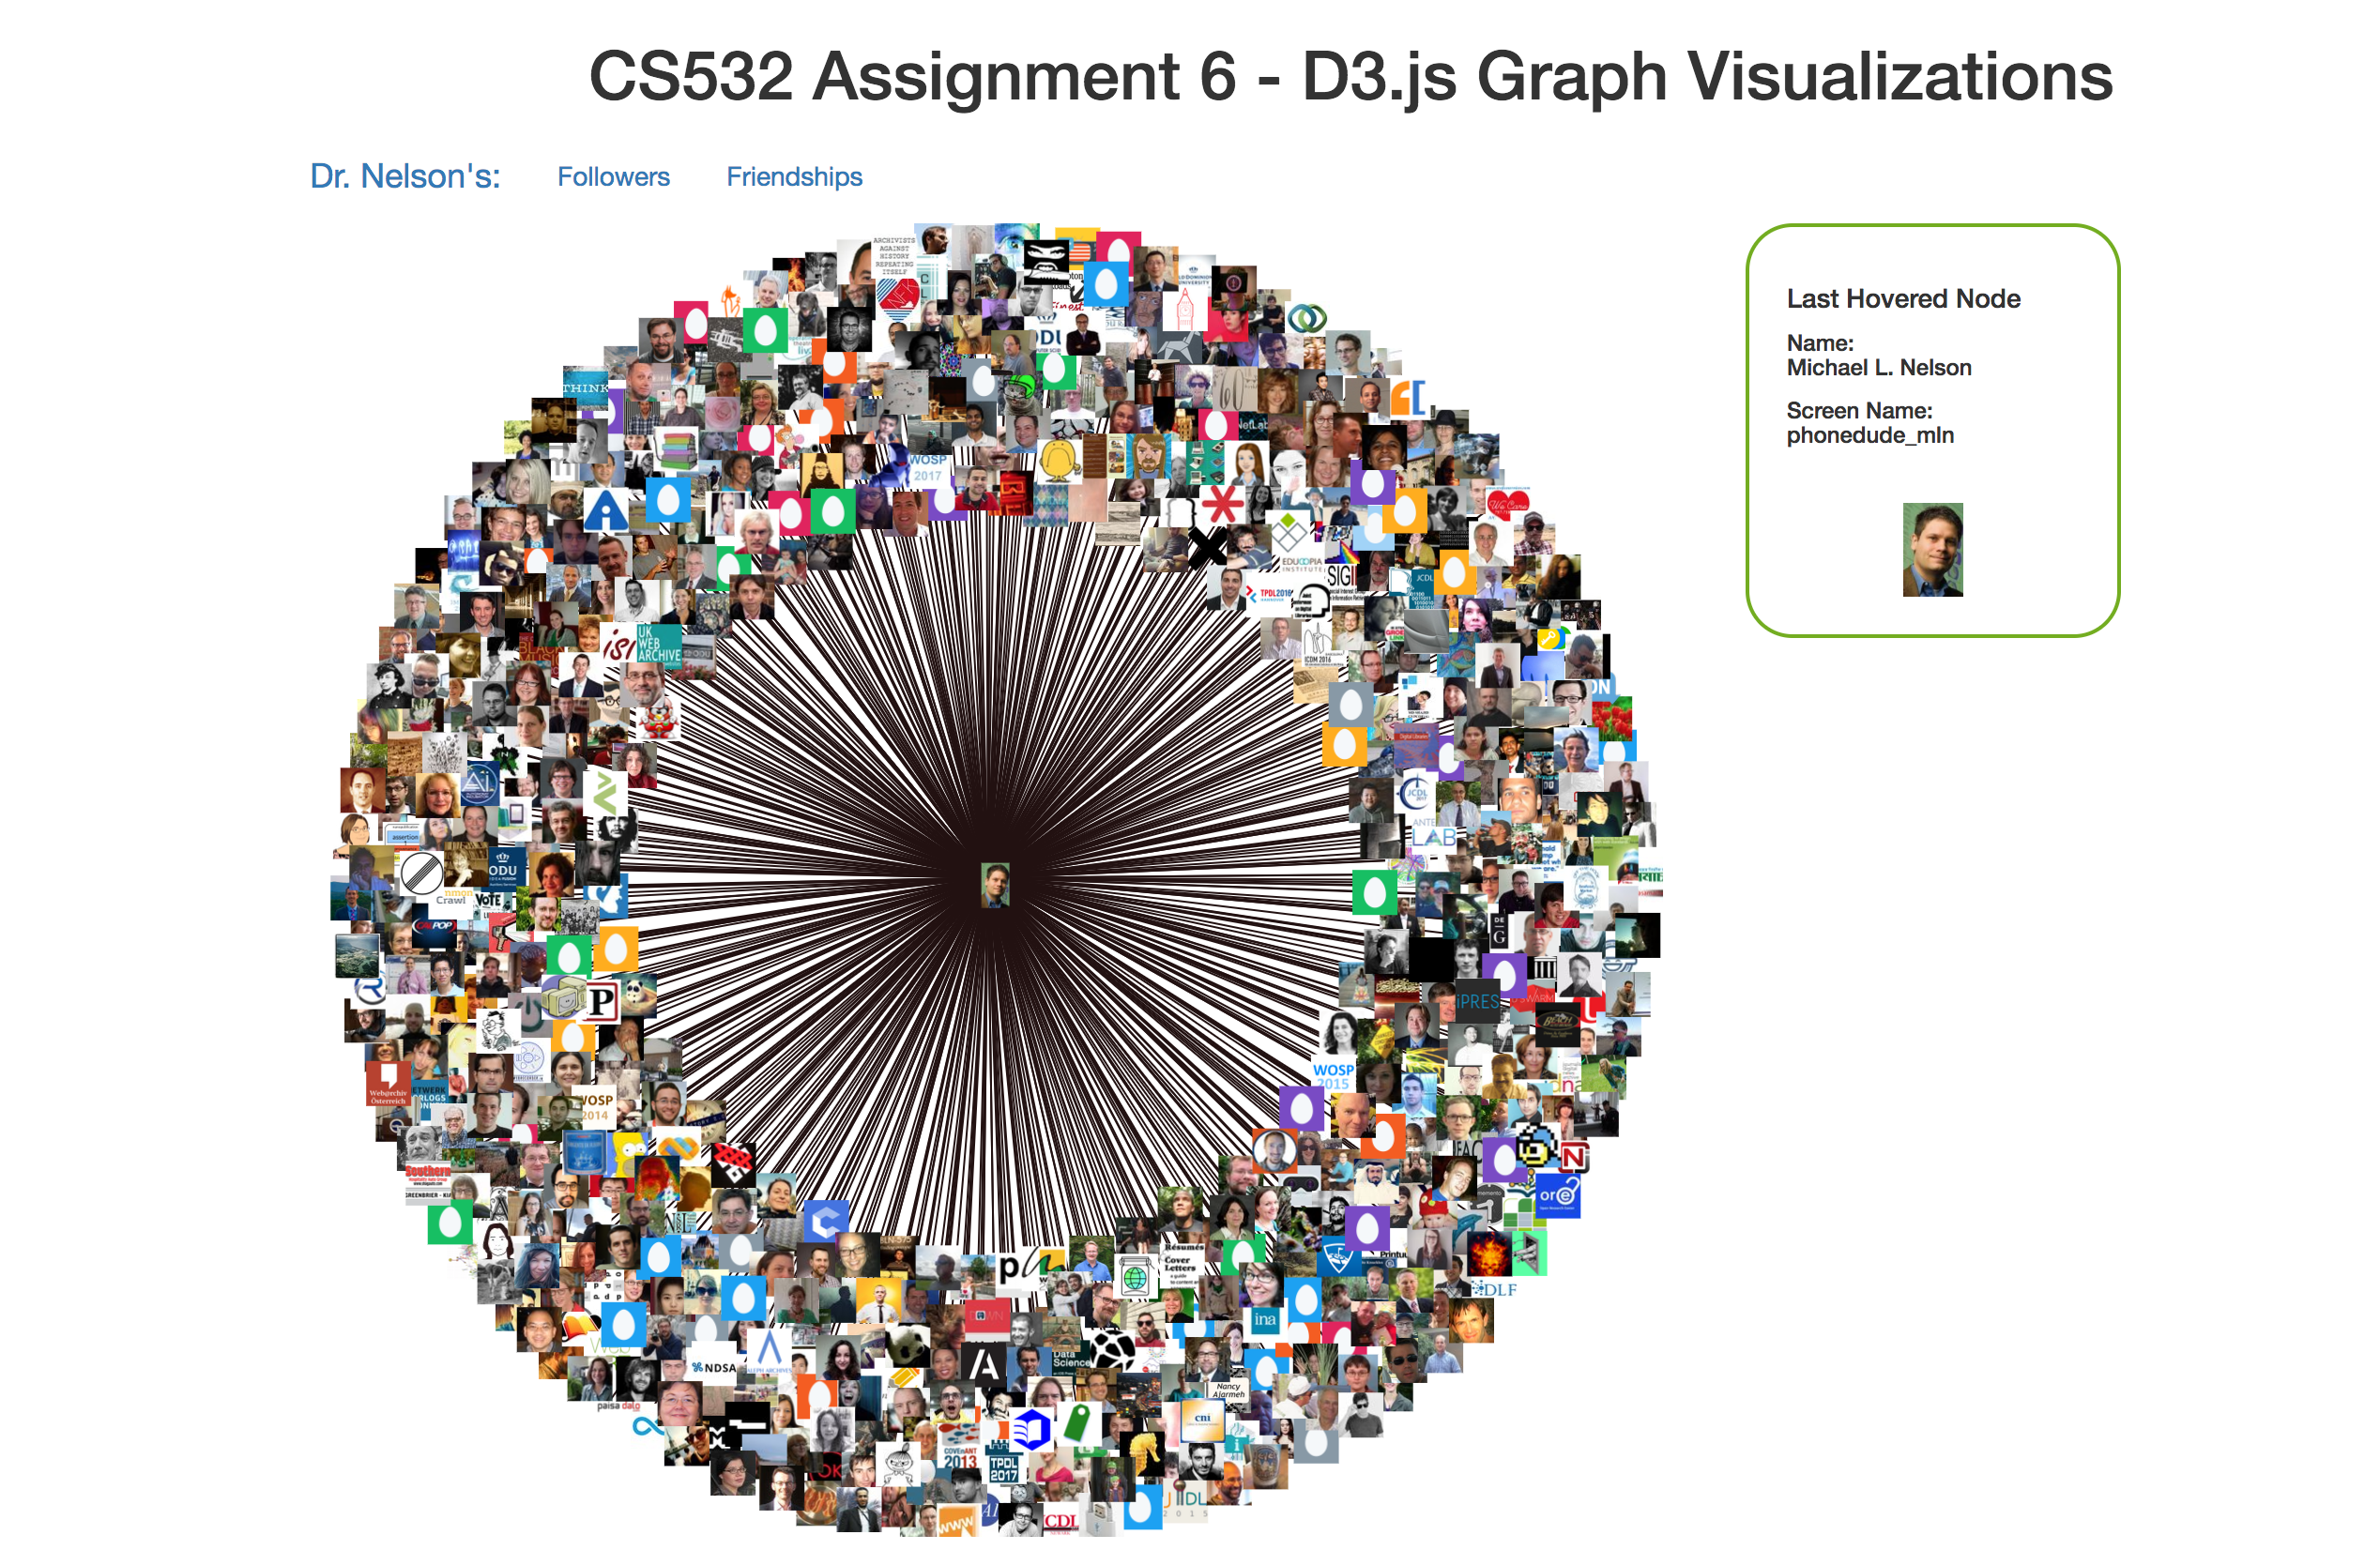
\includegraphics[scale=0.4]{d3followerGraph.png}
 \caption{All of Dr. Nelson's followers in D3 force directed graph}
 \label{fig:q1friendshipgraph}
 \end{figure}

\clearpage
 \begin{figure}[h]
 \centering
 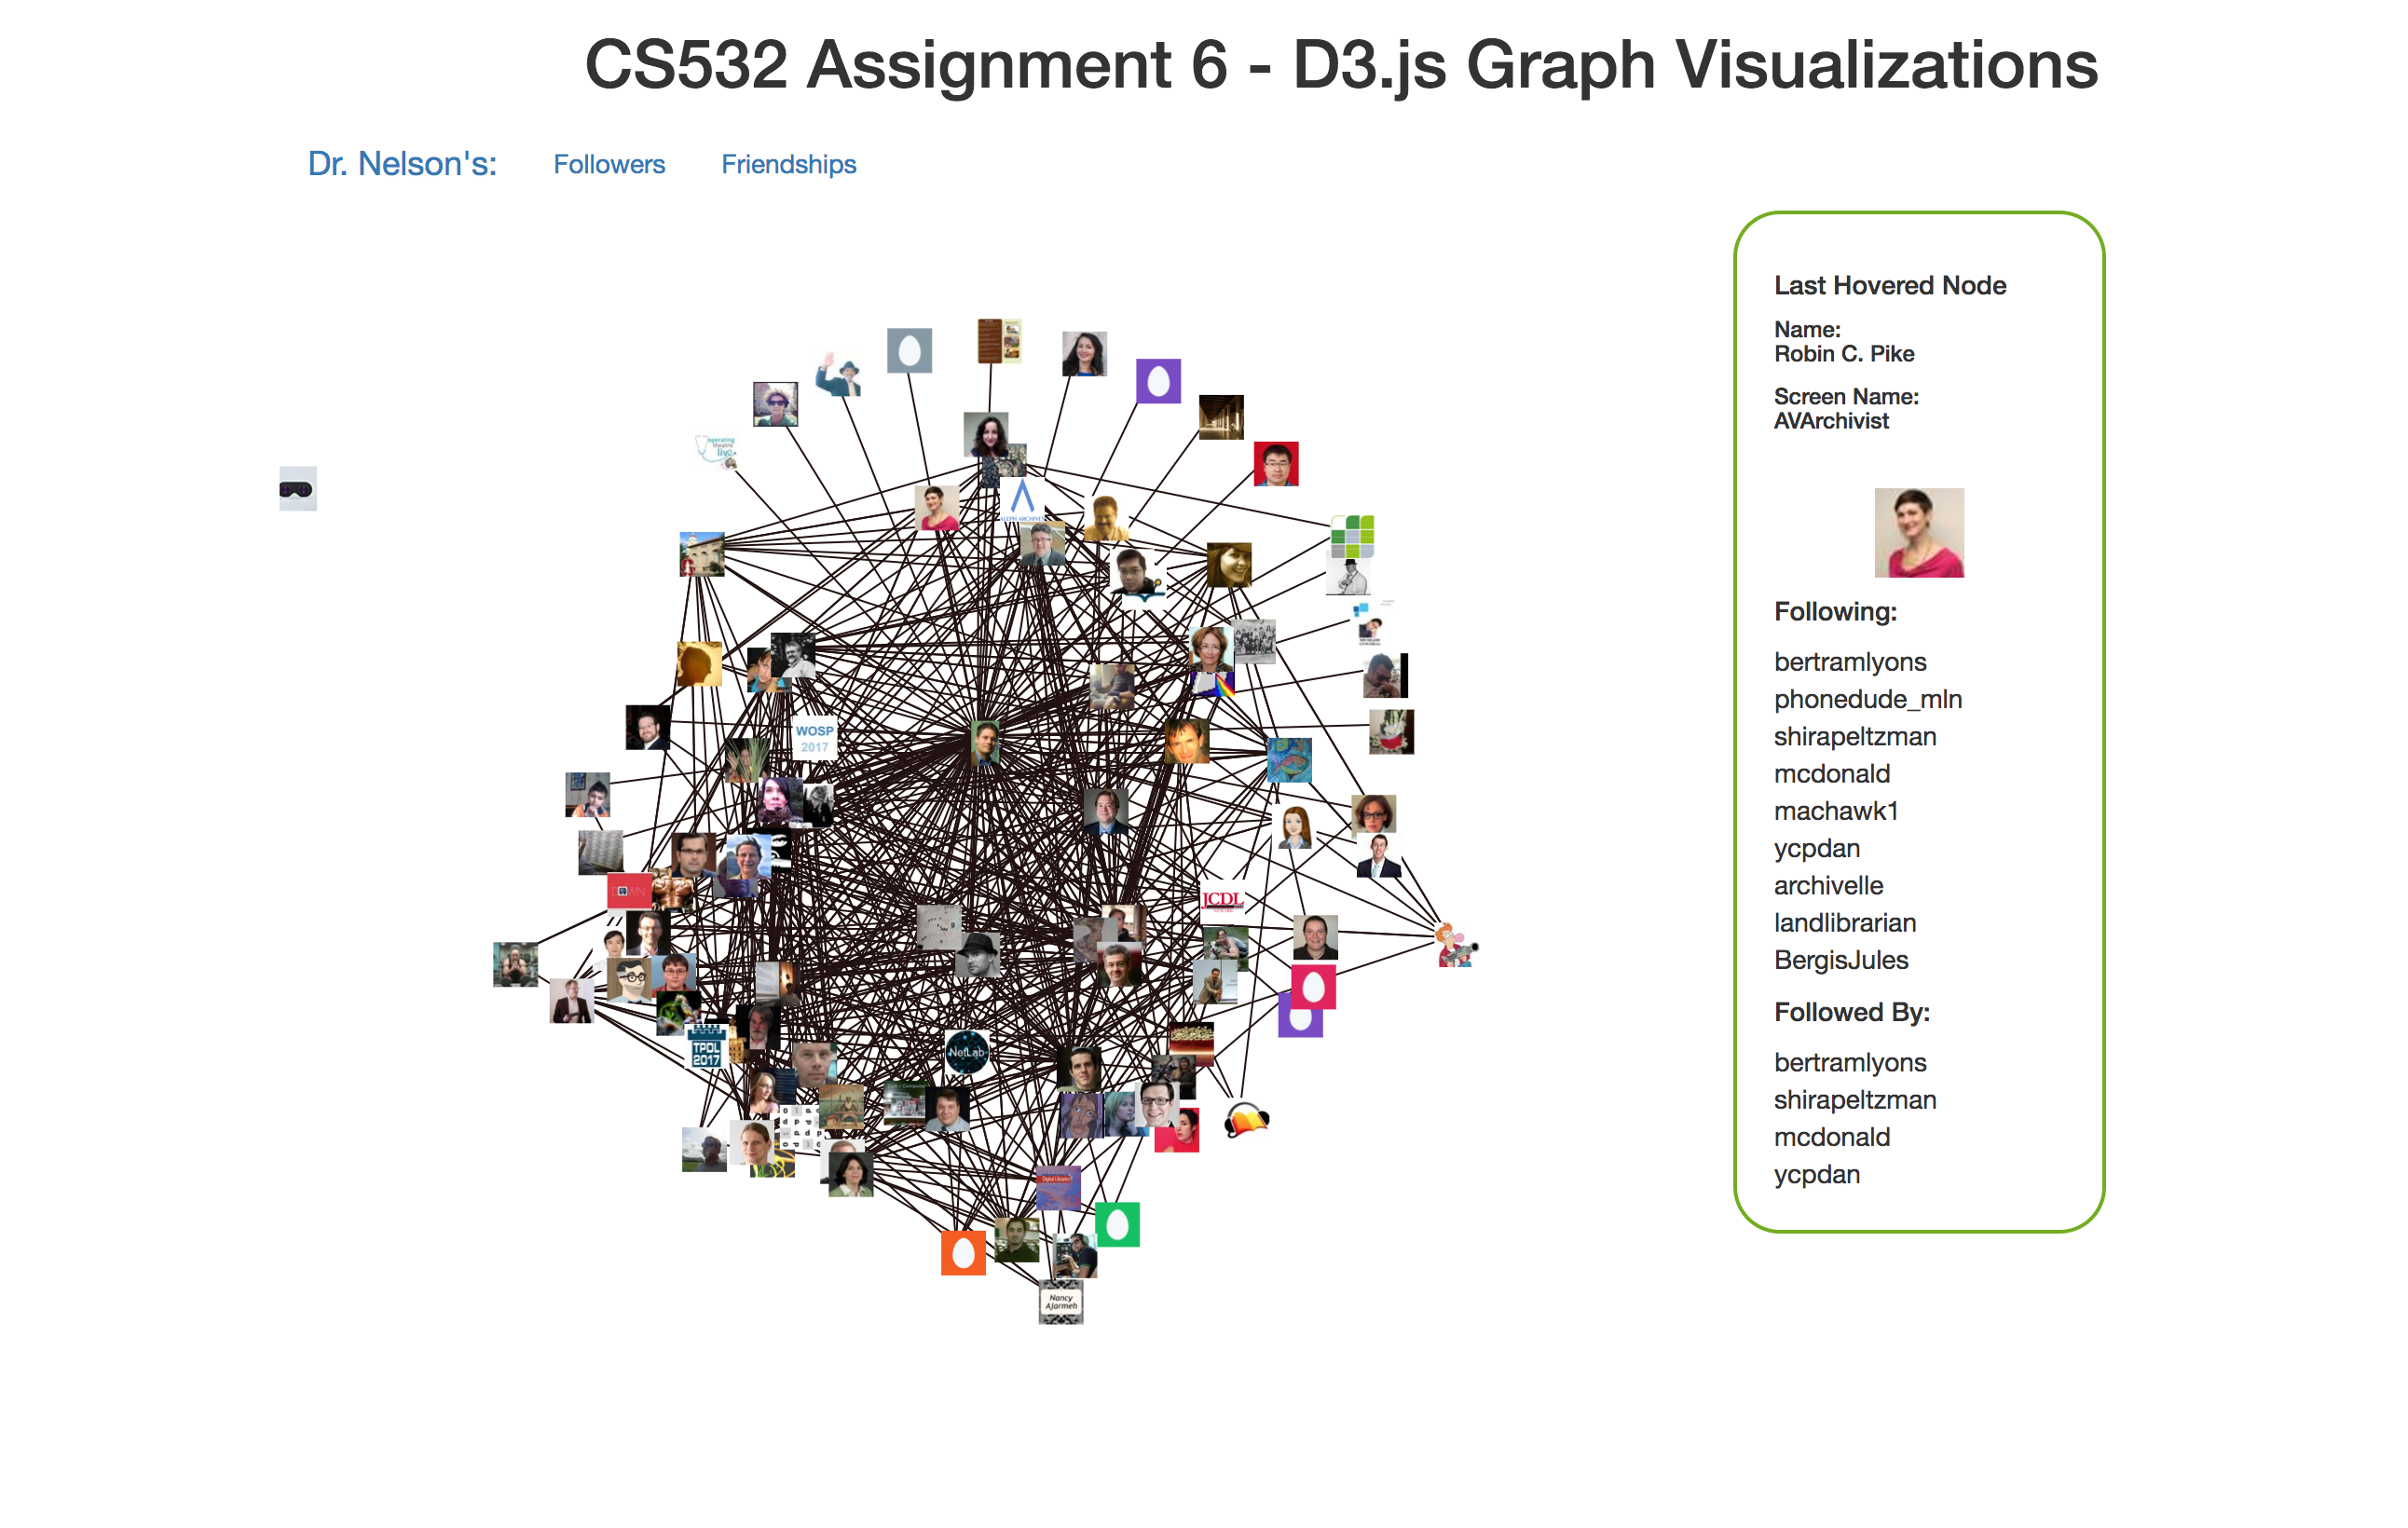
\includegraphics[scale=0.4]{d3friendshipGraph.png}
 \caption{Friendships graph of 100 selected users}
 \label{fig:q1allfollwersgraph}
 \end{figure}

 \lstinputlisting[frame=single,caption={Python script to retrieve Dr. Nelson's followers},label=lst:getFollowers.py,captionpos=b,numbers=left,showspaces=false,showstringspaces=false,basicstyle=\footnotesize]{\srcPath/getFollowers.py}

 \lstinputlisting[frame=single,caption={Python script to check twitter friendships},label=lst:friendships.py,captionpos=b,numbers=left,showspaces=false,showstringspaces=false,basicstyle=\footnotesize]{\srcPath/findFriendships.py}

 \lstinputlisting[frame=single,caption={Javascript to create force directed graphs},label=lst:q1javascript,captionpos=b,numbers=left,showspaces=false,showstringspaces=false,basicstyle=\footnotesize]{\srcPath/js/twitterFriendships.js}

\clearpage

% =================================
% Second question
% =================================

\section*{2}

\subsection*{Question}

\begin{verbatim}
Extra credit: (5 points)

2.  Gender homophily in your Twitter graph 

Take the Twitter graph you generated in question #1 and test for
male-female homophily.  For the purposes of this question you can
consider the graph as undirected (i.e., no distinction between
"follows" and "following").  Use the twitter name (not "screen
name"; for example "Michael L. Nelson" and not "@phonedude_mln")
and programatically determine if the user is male or female.  Some
sites that might be useful:

https://genderize.io/
https://pypi.python.org/pypi/gender-detector/0.0.4

Create a table of Twitter users and their likely gender.  List any 
accounts that can't be determined and remove them from the graph.

Perform the homophily test as described in slides 11-16, Week 8.

Does your Twitter graph exhibit gender homophily?
\end{verbatim}

\subsection*{Answer}

\begin{center}
\Huge{NOT ATTEMPTED}
\end{center}


% \begin{figure}[h]
% \centering
% 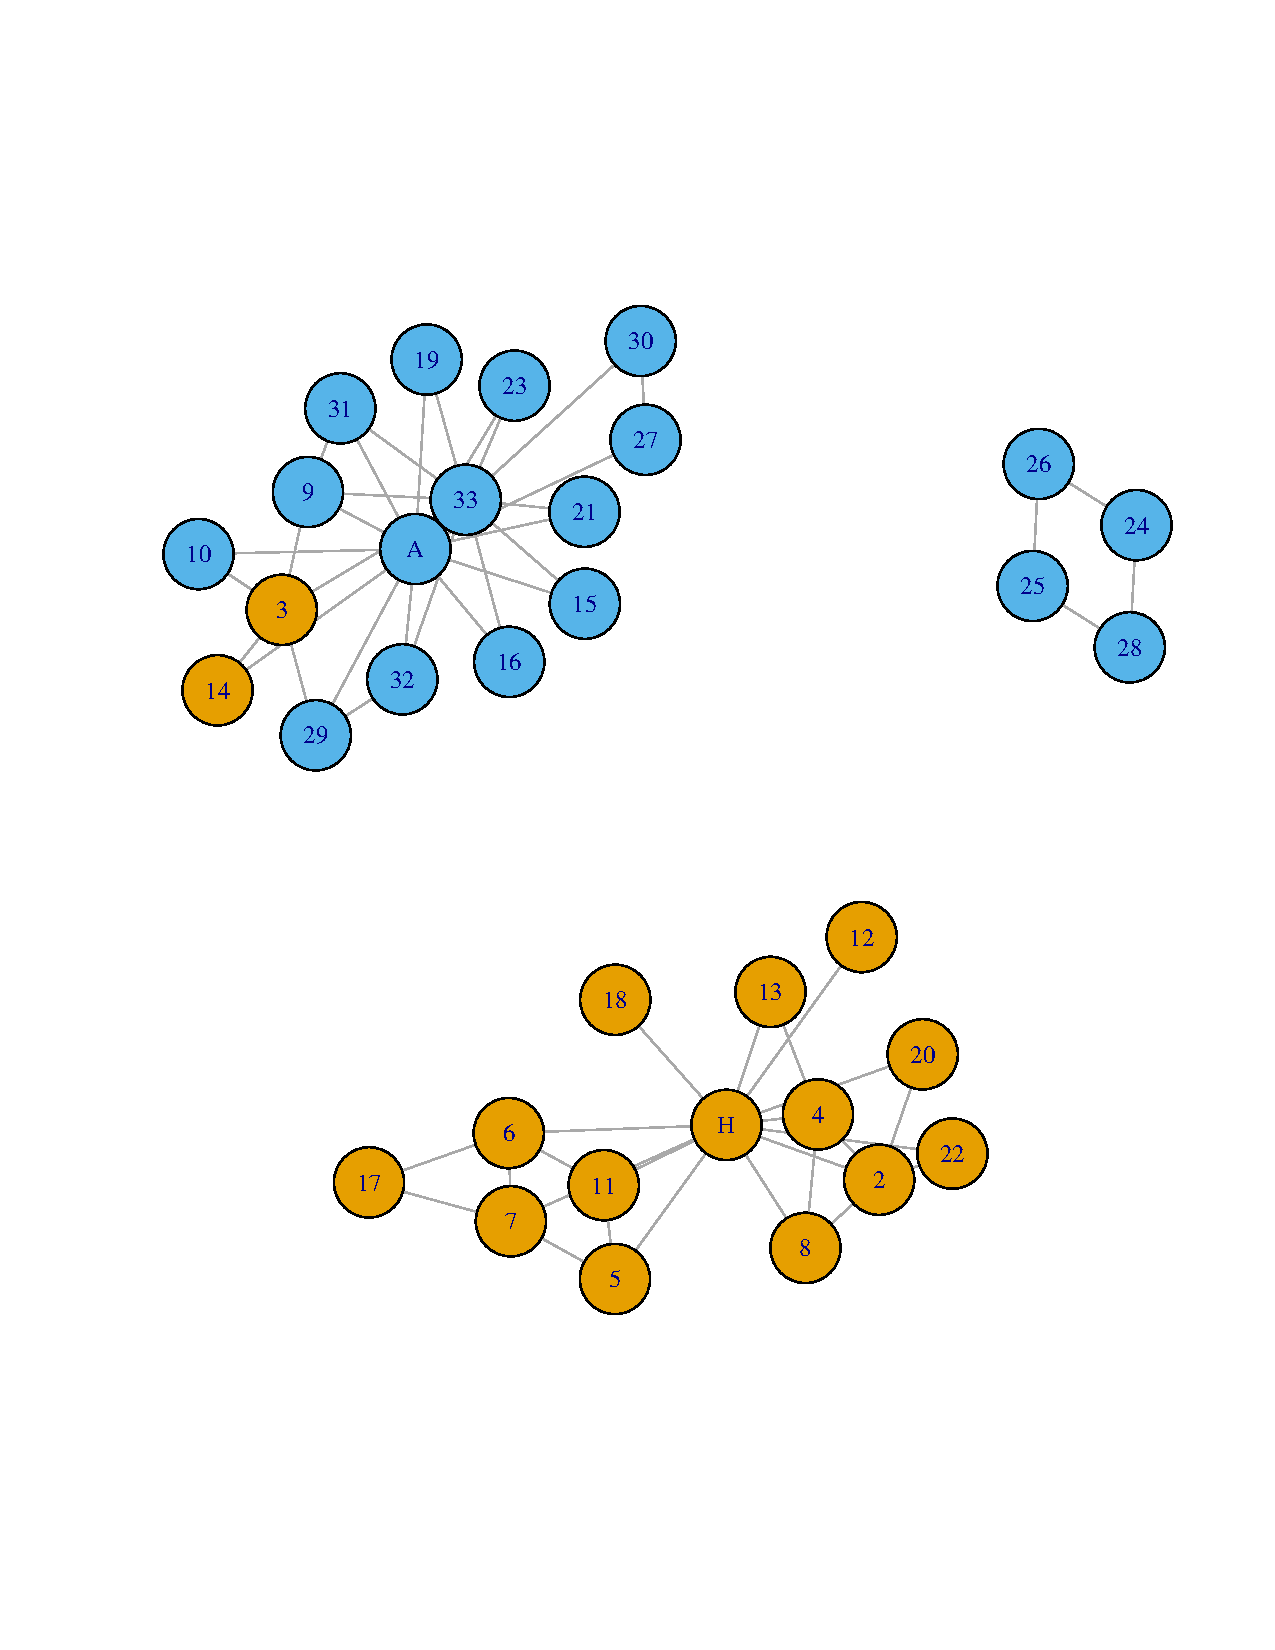
\includegraphics[scale=0.6]{predictedSplit3.pdf}
% \caption{Group split of 3 with Girvan-Newman algorithm from karateClub.R}
% \label{fig:split3}
% \end{figure}

\clearpage

% =================================
% 3rd question
% =================================

\section*{3}

\subsection*{Question}

\begin{verbatim}
Extra credit: (3 points)

3.  Using D3, create a graph of the Karate club before and after
the split.

- Weight the edges with the data from: 
http://vlado.fmf.uni-lj.si/pub/networks/data/ucinet/zachary.dat

- Have the transition from before/after the split occur on a mouse
click.  This is a toggle, so the graph will go back and forth beween
connected and disconnected.
\end{verbatim}

\subsection*{Answer}

\begin{center}
\Huge{NOT ATTEMPTED}
\end{center}

% \begin{figure}[h]
% \centering
% 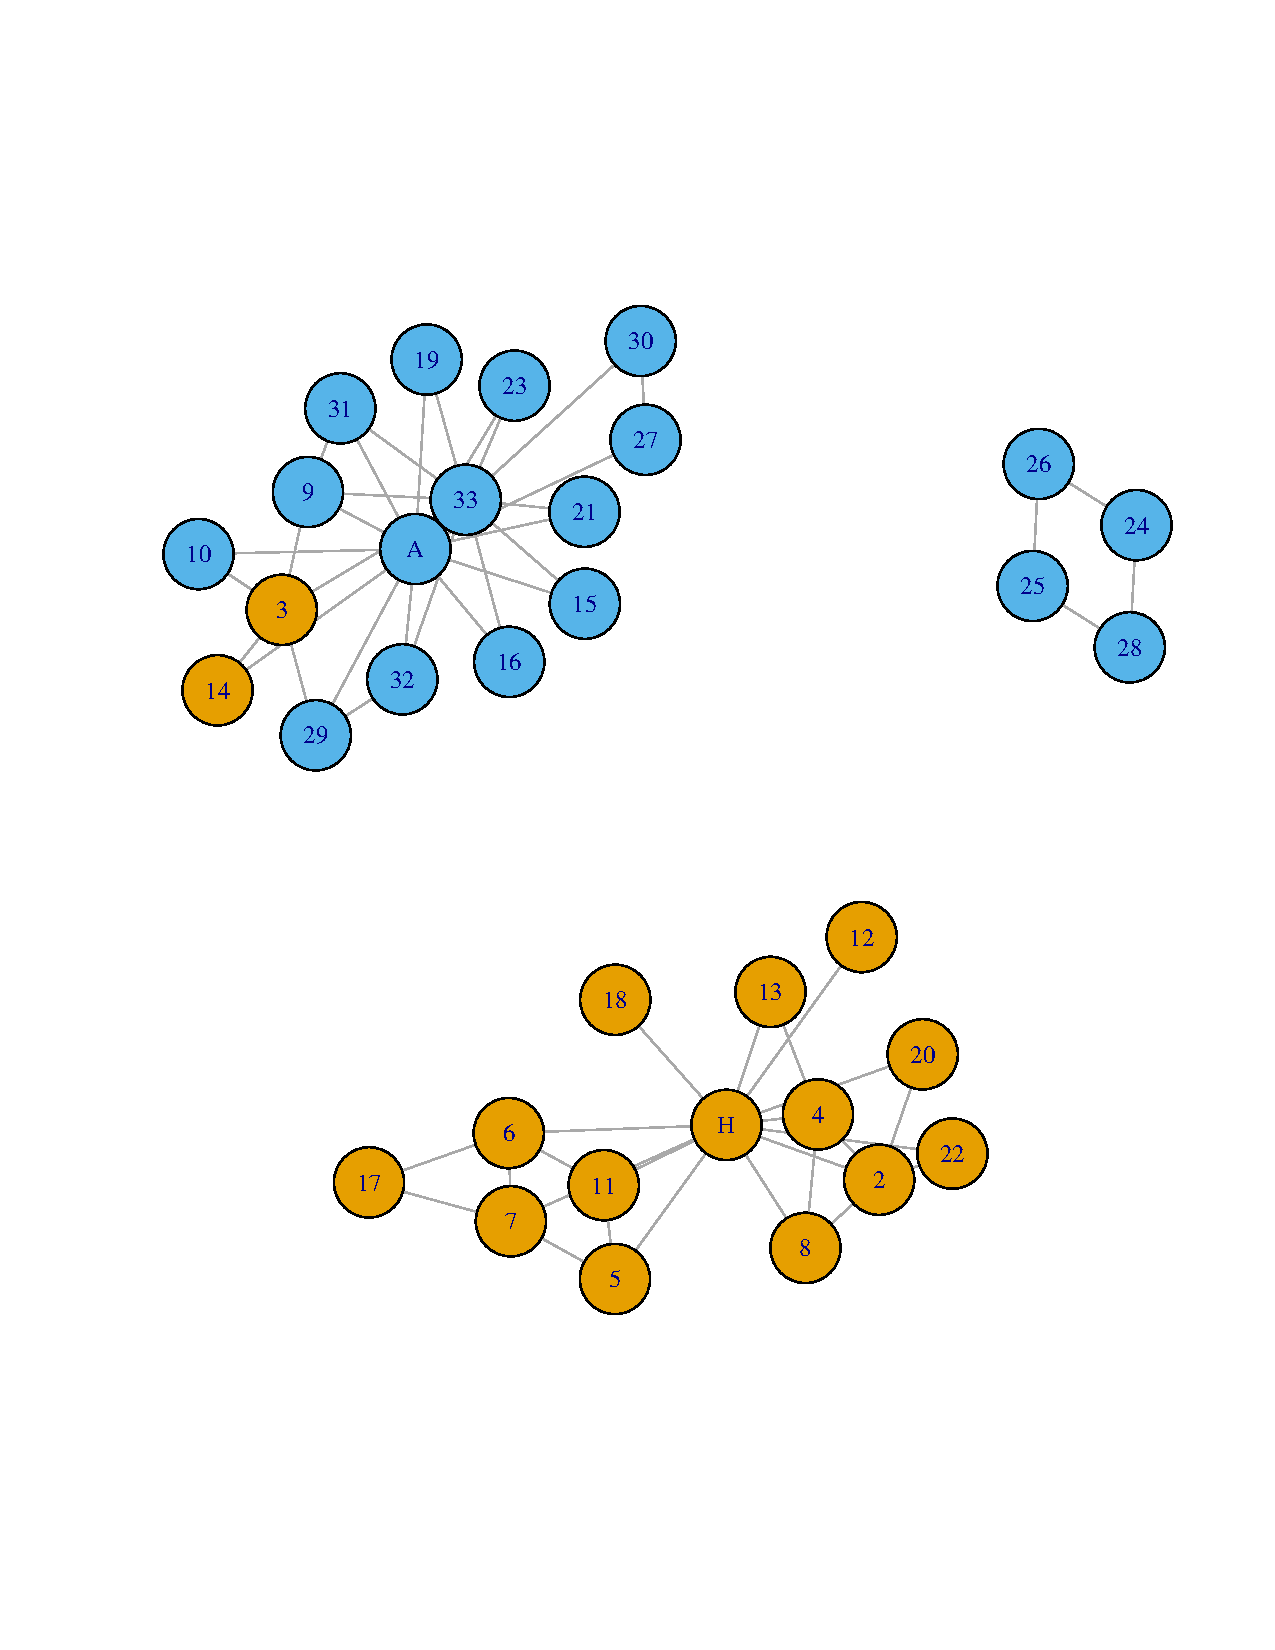
\includegraphics[scale=0.6]{predictedSplit3.pdf}
% \caption{Group split of 3 with Girvan-Newman algorithm from karateClub.R}
% \label{fig:split3}
% \end{figure}

\clearpage

% =================================
% Bibliography
% =================================

\begin{thebibliography}{9}
\bibitem{igraphdataref}
Csardi, Gabor. ``Package `graphdata' '' iGraphData. Cran-R-Project, 13 July 2015. Web. 16 March 2017.\url{https://cran.r-project.org/web/packages/igraphdata/igraphdata.pdf}.
\bibitem{igraphref}
Csardi, Gabor, ``Package `igraph' '' iGraph. Cran-R-Project, 13 July 2015. Web. 16 March 2017. \url{http://igraph.org/r/doc/igraph.pdf}.
\bibitem{commref}
Rodrigues, David.``Finding Communities in networks with R and igraph'' N.p., n.d. Web. 16 March 2017. \url{http://www.sixhat.net/finding-communities-in-networks-with-r-and-igraph.html}.
\bibitem{zachref}
W. W. Zachary, An information flow model for conflict and fission in small groups, Journal of Anthropological Research 33, 452-473 (1977).
\end{thebibliography}

\end{document}